\section{Method}
SEAL executes the program laid out by Sec.~\ref{sec:formulation}: construct a feature space in which Assumption~\ref{as:obs} verifiably holds (Sec.~\ref{sec:feature_engineering}), learn the estimator $f$ with a model whose uncertainty reports where $f=L$ may fail (Sec.~\ref{sec:gpc}), enlarge that region with safe, targeted queries (Sec.~\ref{sec:active}), and deploy $f$ as a runtime invariance monitor over the primitives (Sec.~\ref{sec:supervision}). Fig.~\ref{fig:framework} summarizes the pipeline.

\begin{figure*}[t]
\centering
% TikZ scaffold; thumbnails in Figures/framework_frames/ are LOW-RES CROPS of the
% old framework.png -- regenerate from the original matplotlib outputs (same
% filenames) for print quality. Prompt-template text moved to Appendix~B.
\resizebox{\textwidth}{!}{%
\begin{tikzpicture}[font=\small, >=Latex,
  photo/.style={inner sep=1pt, draw=gray!40, thin},
  blk/.style={rounded corners, draw, thick, align=center, inner sep=3pt,
              minimum height=8mm, font=\small},
  lbl/.style={font=\scriptsize, align=center},
  panel/.style={font=\small\bfseries, anchor=west},
]
% =============== (a) feature engineering (top) ===============
\node[blk, text width=24mm] (prompt)
  {task prompt\\ \scriptsize(Appendix~\ref{app:feature})};
\node[blk, right=8mm of prompt] (llm) {LLM};
\node[blk, right=8mm of llm, text width=22mm] (fsel) {candidate\\ features $F_{\text{sel}}$};
\node[blk, right=8mm of fsel, text width=30mm] (mi)
  {sufficiency check\\ $I(X_{\text{sel}};Y)\ge(1-\epsilon)I(X_{\text{raw}};Y)$};
\node[blk, right=8mm of mi, text width=26mm] (minz)
  {MI minimization:\\ drop redundant\\ features};
\node[blk, right=8mm of minz, fill=teachbg, text width=20mm] (fmin)
  {$F_{\min}$, $\mathcal{X}_{\min}$\\ \scriptsize fixed for all rounds};
\draw[->, thick] (prompt) -- (llm);
\draw[->, thick] (llm) -- (fsel);
\draw[->, thick] (fsel) -- (mi);
\draw[->, thick] (mi) -- node[above, font=\scriptsize]{pass} (minz);
\draw[->, thick] (minz) -- (fmin);
\draw[->, thick, dashed] (mi.south) -- ++(0,-4.5mm) -| node[below, pos=0.25, font=\scriptsize]
  {fail: user refines task description} (prompt.south);
\node[panel] at ([xshift=-2mm,yshift=4mm]prompt.north west)
  {(a) Two-stage feature engineering = observability certificate for Assumption~\ref{as:obs} (Sec.~\ref{sec:feature_engineering})};
% =============== (b) active learning loop (bottom) ===============
\node[photo, below=17mm of prompt.south west, anchor=north west] (demos) {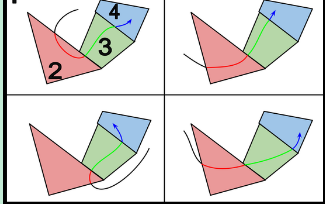
\includegraphics[height=2.1cm]{Figures/framework_frames/demos.png}};
\node[photo, right=13mm of demos] (weak) {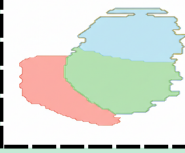
\includegraphics[height=2.1cm]{Figures/framework_frames/weak.png}};
\node[photo, right=13mm of weak] (uncert) {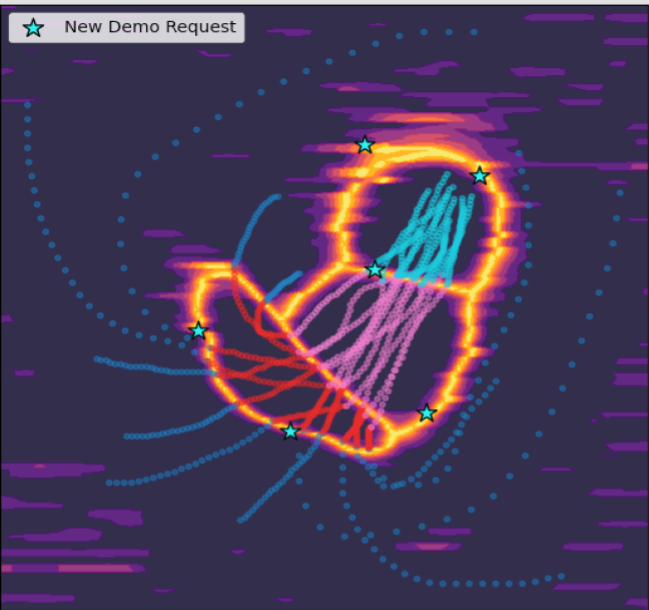
\includegraphics[height=2.1cm]{Figures/framework_frames/uncert.png}};
\node[photo, right=13mm of uncert] (queried) {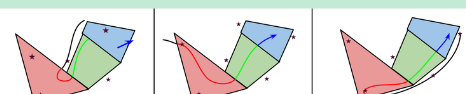
\includegraphics[height=1.35cm]{Figures/framework_frames/queried.png}};
\node[photo, right=13mm of queried] (strong) {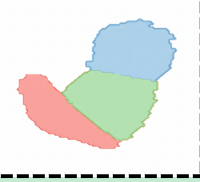
\includegraphics[height=2.1cm]{Figures/framework_frames/strong.png}};
\node[lbl, below=1mm of demos]  {initial segmented\\ demos $\mathcal{D}_0$};
\node[lbl, below=1mm of weak]   {weak classifier};
\node[lbl, below=1mm of uncert] {acquisition $\alpha$,\\ query points $X_K$};
\node[lbl, below=1mm of queried]{safe demos through $X_K$};
\node[lbl, below=1mm of strong] {strong classifier $f$};
\draw[->, thick] (demos) -- node[above, font=\scriptsize]{train} (weak);
\draw[->, thick] (weak) -- (uncert);
\draw[->, thick] (uncert) -- node[above, font=\scriptsize]{\faUser} (queried);
\draw[->, thick] (queried) -- node[above, font=\scriptsize]{retrain} (strong);
\node[panel] at ([xshift=-2mm,yshift=5mm]demos.north west)
  {(b) Active learning of the localizer (Algorithm~\ref{alg:active})};
\end{tikzpicture}%
}

\caption{\textbf{The SEAL pipeline.} (a) An LLM proposes candidate features from the task description; a mutual-information sufficiency check accepts them only if no mode-relevant information was discarded (else the user refines the description), and a minimization pass drops redundant features. The resulting $F_{\min}$ is fixed for all subsequent rounds and at test time. (b) In $F_{\min}$, the initial segmented demonstrations train a weak localizer; the acquisition score selects the states where the guard estimate is least certain, the expert supplies safe demonstrations through them, and retraining yields the deployed localizer $f$ (thumbnails: 2D navigation task of Sec.~\ref{sec:2d_nav}).}
\label{fig:framework}
\end{figure*}

\subsection{Initial Expert Demonstrations}
An expert provides a set of initial demonstrations of the complete task in the raw feature space, yielding $\mathcal{D}_{0,\text{raw}}$. A trajectory is a sequence of feature states $\tau=\{\mathbf{x}_t\}_{t=1}^{T}$, and the expert supplies dense, per-point mode labels by emitting a trigger signal upon completion of each subtask. Once the minimal feature set $F_{\min}$ is determined (Sec.~\ref{sec:feature_engineering}), the raw data is processed into a working dataset of $N$ labeled trajectories,
\begin{equation}
\mathcal{D}_{0,\text{min}}=\{(\tau_i,\ell_i)\}_{i=1}^N
\;\equiv\;\bigcup_{i=1}^{N}\bigcup_{t=1}^{T_i}\{(\mathbf{x}_{i,t},m_{i,t})\},
\end{equation}
where $\ell_i=\{m_{i,t}\}_{t=1}^{T_i}$ are the per-point mode labels and the right-hand side is the flattened point set on which the classifier trains. These demonstrations are not overhead specific to the classifier: being successful expert trajectories, they can double as training data for the low-level primitives. (To isolate the mode supervisor, our experiments use programmatic primitives.) The only additional cost is the per-segment trigger signal, which we validate as negligible in Sec.~\ref{sec:user_study}. We assume all initial demonstrations adhere to valid transitions and complete the task successfully.

\subsection{Two-Stage Feature Engineering as an Observability Certificate}
\label{sec:feature_engineering}
The localizer must operate in a space where every sampled point is physically realizable and interpretable for expert labeling; a sample drawn in raw pixel space is neither. We therefore work with grounded features (object poses, relations). However, even a few absolute object poses push the dimension above ten, which is problematic for two reasons: the curse of dimensionality inflates the demonstrations needed for dense coverage, and the physically valid manifold occupies a vanishing fraction of the ambient space, so uncertainty-driven sampling (Sec.~\ref{sec:active}) frequently proposes infeasible configurations (objects suspended in mid-air) that an expert cannot demonstrate. We reduce the space with a two-stage pipeline (Fig.~\ref{fig:framework}a) that also \emph{certifies} Assumption~\ref{as:obs}.

Notation: $F_{\text{raw}}$ denotes the full set of \emph{grounded observables} exposed by the perception stack (object poses, gripper status, and quantities derivable from them); ``raw'' in the sense of \emph{unselected}, not unprocessed; pixel-level state is already excluded. For any feature set $F$, evaluating its functions along the demonstrations yields the data matrix $X_F$; we write $X_{\text{raw}}$, $X_{\text{sel}}$, $X_{\min}$ for the data under $F_{\text{raw}}$, $F_{\text{sel}}$, $F_{\min}$. Selection acts on features; the MI estimator acts on data.

\textbf{Stage 1: Semantic generation.} An LLM~\cite{gemini} acts as a semantic prior. Prompted with the task description, the available features $F_{\text{raw}}$, and target modes, it outputs a candidate set $F_{\text{sel}}$ that penalizes absolute coordinates in favor of spatially invariant relative metrics. We map the demonstrations into $X_{\text{sel}}$ and estimate the joint mutual information $I(X_{\text{sel}};Y)$ against the discrete mode labels $Y$ using a $k$-nearest-neighbor estimator for mixed continuous--discrete data~\cite{10.1371/journal.pone.0087357}. If $I(X_{\text{sel}};Y)$ falls short of the raw baseline $I(X_{\text{raw}};Y)\approx H(Y)$ by more than a tolerance $\epsilon$ (we accept when $I(X_{\text{sel}};Y)\ge(1-\epsilon)\,I(X_{\text{raw}};Y)$, with an empirical tolerance of $\epsilon = 0.01$), the LLM has discarded mode-relevant information; the system rejects $F_{\text{sel}}$ and asks the user for a more detailed description. This test is exactly the empirical observability certificate of Assumption~\ref{as:obs}.

\textbf{Stage 2: Mathematical minimization.} Given a sufficient $F_{\text{sel}}$, we prune redundancy by evaluating lower-dimensional projections (dropping feature columns and recomputing the MI) and define $X_{\min}$ as the lowest-dimensional projection that preserves the baseline MI, with corresponding features $F_{\min}$. If no feature is redundant, $F_{\min}=F_{\text{sel}}$. {\color{blue}Features the LLM nominated as failure-relevant are exempt from this pruning and retained regardless of their nominal MI, since a variable that is near-constant across success-only demonstrations (e.g., payload presence) can still be decisive at a failure boundary (Remark~\ref{rem:aliasing}). [INTERNAL, discuss: this states the exemption the aliasing Remark already commits to, and supersedes the earlier ``I could not come up with an example'' rebuttal --- the Remark's payload-presence case is exactly such a feature. Confirm the code actually retains these features, or soften Remark~\ref{rem:aliasing}.]} Because MI alone cannot distinguish causal geometry from spurious spatial correlation in the few-shot regime (Appendix~\ref{app:feature}), the LLM's invariance prior is what makes the resulting space causally robust; MI supplies the sufficiency and minimality guarantees. In all later rounds, new data is processed directly into $F_{\min}$.

\subsection{Localization via a Gaussian Process Classifier}
\label{sec:gpc}
We instantiate $f$ as a Gaussian Process Classifier (GPC) for its decomposable uncertainty, which is central both to active learning and to confidence-gated switching. A GPC defines a distribution over latent functions; the posterior predictive for a test point $\mathbf{x}^*$ is
\begin{equation}
P(m\mid\mathbf{x}^*,\mathcal{D}_{k})=\int\sigma(f^*)\,p(f^*\mid\mathcal{D}_{k})\,df^*,
\end{equation}
with $\sigma(\cdot)$ the softmax link and $p(f^*\mid\mathcal{D}_{k})$ the (non-Gaussian) latent predictive distribution. The integral is intractable, so we approximate the posterior by a Gaussian $q(\mathbf{f})$ via variational inference using GPyTorch~\cite{gardner2018gpytorch} with $M$ inducing points, where $M$ scales with the dataset size but is capped; inference then completes in a few milliseconds per step, fast enough for low-latency monitoring. Implementation details and a calibration analysis of the resulting confidences are given in Appendix~\ref{app:ablation}.

\textbf{Mixed continuous--discrete features.} Robotic states mix continuous variables $\mathbf{x}_{\text{cont}}\in\mathbb{R}^d$ (relative distances) with discrete ones $c\in\mathbb{N}$ (e.g., gripper status). A single RBF kernel over the joint space assumes context-independent correlation, while separate classifiers per discrete value waste data. We use a product kernel
\begin{equation}
k(\mathbf{x},\mathbf{x}')=k_{\text{RBF}}(\mathbf{x}_{\text{cont}},\mathbf{x}'_{\text{cont}})\cdot k_{\text{idx}}(c,c'),
\end{equation}
where the index kernel $k_{\text{idx}}$ learns a low-rank covariance $\mathbf{B}$ across discrete contexts. Unlike a fixed Kronecker delta, a learnable $\mathbf{B}$ lets the GPC share information across contexts when useful or isolate them when not, and it scales to more than two discrete contexts where per-context models become data-hungry (Appendix~\ref{app:ablation}). During candidate selection we fix the discrete variables and sample the continuous space.

\subsection{Uncertainty-Targeted Active Learning}
\label{sec:active}
The GPC exposes \emph{epistemic} uncertainty (ignorance in low-density regions), distinct from \emph{aleatoric} boundary ambiguity. As a proxy we use the summed latent variance across modes, which is large wherever data is sparse (though it does not separate the two sources perfectly near guards),
\begin{equation}
\eta(\mathbf{x}^*)=\sum_{m\in\mathcal{M}}\text{Var}(f^*_m).
\end{equation}
Because raw epistemic uncertainty peaks at the extreme edges of the state space, we weight it by a centring prior $W(\mathbf{x}^*)$, a Gaussian over the workspace whose mean and covariance are set once from the spread of $\mathcal{D}_{0}$ (not tuned per task). The acquisition score is
\begin{equation}
\alpha(\mathbf{x}^*)=\eta(\mathbf{x}^*)\cdot W(\mathbf{x}^*).
\end{equation}
The learning loop is summarized in Algorithm~\ref{alg:active} and illustrated in Fig.~\ref{fig:framework}b. Batch diversity uses greedy furthest-point sampling on standardized features (so that meters, radians, and binary flags are comparable),
\begin{equation}\label{eq:sampling}
\mathbf{x}_k=\operatorname*{argmax}_{\mathbf{x}\in\mathcal{U}_{\text{top}}\setminus X_{k-1}}\ \min_{\mathbf{x}_j\in X_{k-1}}\|\mathbf{x}-\mathbf{x}_j\|_2,
\end{equation}
initialized at $\mathbf{x}_1=\arg\max_{\mathbf{x}}\alpha(\mathbf{x})$. The candidate grid is feasible precisely because Sec.~\ref{sec:feature_engineering} has reduced the space to a few dimensions. Because the features are grounded (object poses, relations), each queried point is realized physically: the scene is configured to match the queried feature state (e.g., the spray bottle is laid on its side at the queried offset), and the expert demonstrates from there, supplying \emph{prescriptive} labels: the mode that should be executed from that state to advance the task. Our experiments use a single active round.

\begin{algorithm}
\caption{Uncertainty-Targeted Active Learning}\label{alg:active}
\begin{algorithmic}[1]
\Require initial demos $\mathcal{D}_{0}$, batch size $K$, rounds $R$
\For{$k=0,\dots,R-1$}
\State train GPC $f$ on $\mathcal{D}_{k}$
\State compute $\alpha(\mathbf{x})=\eta(\mathbf{x})\,W(\mathbf{x})$ on a dense grid over the bounding box of $\mathcal{D}_{0}$
\State $\mathcal{U}_{\text{top}}\gets$ top decile of $\alpha$
\State $X_K\gets K$ diverse points from $\mathcal{U}_{\text{top}}$ via Eq.~\eqref{eq:sampling}
\State configure scenes at $X_K$; expert provides safe, segmented demos $\mathcal{D}_{\text{new}}$
\State $\mathcal{D}_{k+1}\gets\mathcal{D}_{k}\cup\mathcal{D}_{\text{new}}$
\EndFor
\State \Return $f$ trained on $\mathcal{D}_{R}$
\end{algorithmic}
\end{algorithm}

\subsection{Confidence-Gated Supervision}
\label{sec:supervision}
Once trained, $f$ acts as a supervisory layer over the primitives $\{\pi_m\}$ with nominal sequence $S$. The two signals are kept deliberately separate, and $f$ is deliberately \emph{memory-less}. Its purpose is to serve as an independent check on $S$: were $f$ to condition on the history of modes visited, it would implicitly re-learn a prior over $S$ itself (every demonstration shows only the nominal order), and its disagreement with $S$ would become correlated with $S$ precisely at the moment of an anomalous transition, when independence matters most. Concretely, a history-conditioned localizer such as an HMM updates its belief as $\mathrm{Belief}(S_t)\propto P(O_t\mid S_t)\sum_{S_{t-1}} P(S_t\mid S_{t-1})\,\mathrm{Belief}(S_{t-1})$; since the demonstrations contain only nominal transitions, the learned prior $P(S_t\mid S_{t-1})$ is near zero for exactly the anomalous transition a failure induces, so even a high observation likelihood $P(O_t\mid S_t)$ cannot move the estimate onto the failed mode, and a majority-vote filter over $f$ only adds latency. Estimating the mode from the instantaneous state alone keeps the monitor's failure signal decoupled from the sequence logic it supervises. The execution logic is given in Algorithm~\ref{alg:supervision}. At each step the classifier localizes the current mode $m^*$ with confidence $prob^*$; a non-nominal mode overrides the current one only if it is both confident ($prob^*>\tau$ where we empirically set $\tau = 0.80$ across all tasks to balance false positives and reaction time) and persistent (holds for $N_{\text{thresh}}$ consecutive steps). The persistence counter $N_{\text{thresh}}$ is a \emph{dwell-time} condition that prevents chattering across a guard surface; unlike a fixed debounce buffer, confidence gating lets us keep $N_{\text{thresh}}$ small and instead reject \emph{low-confidence} switches, so that genuine transitions, which push the state deep into a neighboring region where confidence is high, are honored quickly (Sec.~\ref{sec:scooping}).

\begin{algorithm}
\caption{Confidence-Gated Mode Supervision}\label{alg:supervision}
\begin{algorithmic}[1]
\Require GPC $f$, nominal sequence $S$, confidence threshold $\tau$, dwell $N_{\text{thresh}}$
\State $m_{\text{current}}\gets\text{first mode in }S$
\While{task is not complete}
\State $\mathbf{x}_t\gets\text{extract features }F_{\min}\text{ at time }t$
\State $m^*, prob^*\gets f(\mathbf{x}_t)$ \Comment{localize current mode + confidence}
\If{same $m^*\neq m_{\text{current}}$ \textbf{with} $prob^*>\tau$ for $N_{\text{thresh}}$ consecutive steps}
    \State $m_{\text{current}}\gets m^*$ \Comment{confident, persistent recovery}
\EndIf
\State \textbf{Execute} step of $\pi_{m_{\text{current}}}(\mathbf{x}_t)$
\If{$\pi_{m_{\text{current}}}$ signals completion}
    \State $m_{\text{current}}\gets\text{next mode in }S$ \Comment{nominal advance}
\EndIf
\EndWhile
\end{algorithmic}
\end{algorithm}

%%%%%%%%%%%%%%%%%%%%%%%%%%%%%%%%%%%%%%%%%%%%%%%%%%%%%%%%%%%%%%%%%%%%%%%%%%%%%%%%
